\chapter{Requisitos y oficina física}\label{S:anexo_B}
Este anexo contiene las explicaciones, comparativas y conclusiones parciales relacionadas con la creación de una oficina física, hardware así como la documentación fotográfica y otros detalles de la implementación real de “mi oficina” como desarrollo práctico del capítulo \ref{S:tema_1}.

\section{Definición y tipos de requisitos}\label{S:requisitos}

Definición de “\textbf{mínimo}”, entendemos un requisito de mínimos aquellos que permiten realizar el trabajo no exentos de problemática y repercutiendo en la performance o agilidad durante el trabajo. Ejemplos que permiten trabajar de manera “mínima” son aquellos donde tenemos un pc/laptop  y una o varias de las siguientes casuísticas:
\begin{itemize}
    \item Mesa y silla, no especializada y compartida para otros usos.
    
    \item Un pc/laptop que no cumple los requisitos mínimos para hacer el trabajo de manera holgada y afecta negativamente tanto en su uso como en el tiempo requerido.
    
    \item Un espacio de trabajo compartido, ruidoso, con constantes interrupciones ajenas al desarrollo profesional.
    
    \item Conexión de internet insuficiente, que limita las comunicaciones y retrasa significativamente el trabajo.
    
\end{itemize}

Definición de “adecuado”, este apartado puede variar en función de la especialización del trabajo a realizar. Mientras un soporte de incidencias necesita de unos requisitos de hardware básicos, buena conectividad; un renderizado de imagen/vídeo puede necesitar de un hardware potente y una conexión mediocre. Por lo tanto, se sobreentiende que la definición promedio debe estar sensiblemente acoplada a la actividad a realizar. Como se ha mencionado en nuestro contexto nos focalizamos en la creación o gestión de software.

Un  requisito “\textbf{adecuado}” debe permitir una mejora sustancial del 30-40\% en las tareas a realizar sobre un requisito de “mínimo” y permitir evitar la gran mayoría de puntos negativos, que pueden degradar o repercutir no solo la realización y calidad de trabajo sino las comodidad y satisfacción del trabajador.

Un  requisito “\textbf{óptimo}”, depende en gran medida de la especialización y los gustos del propio trabajador, incrementa normalmente la satisfacción del trabajador aunque no es una mejora sustancial en la productividad del trabajo intrínseco.

De una manera muy similar podemos hablar de 4 amalgamas presupuestarias, “\textbf{básico}” usualmente acoplada a la definición de “\textbf{mínimo}”, “\textbf{profesional}” focalizada en calidad precio cumpliendo los requisitos de “\textbf{adecuado}”, “\textbf{profesional pro}” excede los requisitos de adecuado y se acerca a “\textbf{óptimo}” a un precio justificado y finalmente “\textbf{business}”, excede no sólo los requisitos de óptimo y normalmente malgasta recursos o opta por acabados y marcas de mayor prestigio que no aportan mejoras medibles.

\section{Requisitos físicos}

Este apartado evalúa y compara diferentes niveles mínimos/adecuados/óptimos como requisito físicos, es decir, elementos de hardware, espacio e instalaciones para la realización de un trabajo profesional.

\subsection{Área de Trabajo}
Un cubículo público como el que podemos encontrar en las bibliotecas de la UPC (fig. \ref{F:cubiculo_upc}) es el área de trabajo mínima. Un área de trabajo de menos de 1 metro cuadrado capaz de almacenar un portátil y documentación auxiliar, conectividad WIFI, alimentación eléctrica, una silla y como se aprecia en la imagen un área personal aprox. de otro metro cuadrado que en muchos casos delimitada por biombos, marquesinas o cristales translúcidos. 

\begin{figure}[htb]
\begin{center}
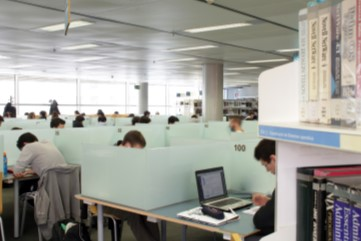
\includegraphics[width=0.75\textwidth]{./figuras/cubiculo_upc}
\caption{Cubículo biblioteca UPC (campus nord)}
\label{F:cubiculo_upc}
\end{center}
\end{figure}

El objetivo de esta área no solo es soportar los elementos de trabajo, sino aislar de distracciones o interacción social al trabajador. Usaremos este cubículo como definición mínima, duplicaremos los requisitos para adecuada y generalizamos en una habitación o pseudo habitación reservada como óptima.

Iluminación artificial (mínimo), compaginada con luz natural (adecuado), luz regulable, persianas, estores, tanto natural como artificial (óptima).

 Ventilación diaria manual (mínimo), ventilación natural o automática (adecuado), espacio aclimatado con filtros, regulador de humedad y porcentaje de aire externo (óptimo).

 \subsection{Otros elementos}

 Es de importancia significativa la selección de mobiliario y elementos auxiliares tales como alfombrillas (mínimo), mesa o escritorio no especializadas (mínimo), escritorio de más 70 cm de altura o regulable (adecuado), mesa-escritorio especializada motorizada que permite trabajar de pie (óptimo).

\begin{figure}[htb]
\begin{center}
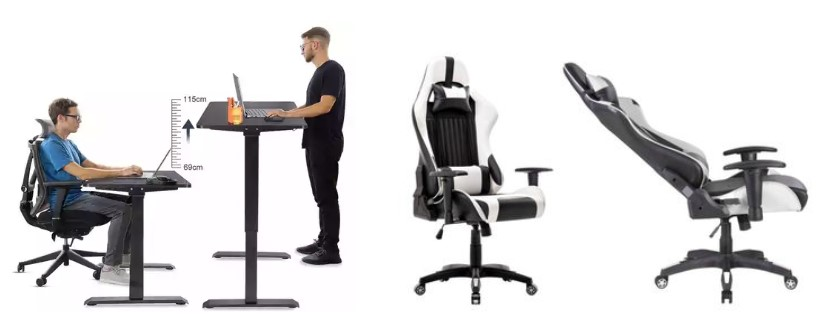
\includegraphics[width=1\textwidth]{./figuras/amazon_sillas}
\caption{Silla y mesas, productos Amazon.}
\label{F:amazon_sillas}
\end{center}
\end{figure}

Silla ergonómica básica (mínimo), silla ergonómica ajustable con cojín lumbar (adecuado), silla gamer o business (óptimo).

\begin{figure}[htb]
\begin{center}
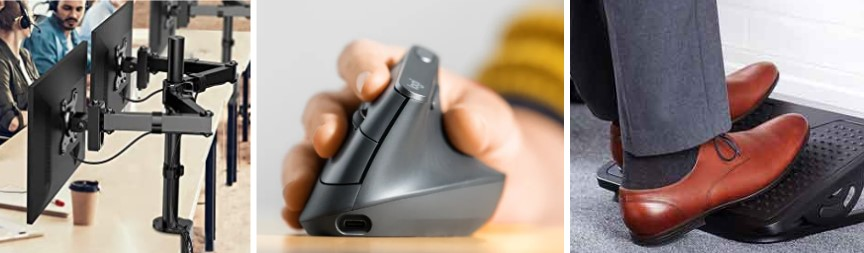
\includegraphics[width=1\textwidth]{./figuras/amazon_extras}
\caption{Porta monitor, raton ergonómico, productos Amazon.}
\label{F:amazon_extras}
\end{center}
\end{figure}

Elemento opcionales como, reposapiés (adecuado), ratón ergonómico / almohadilla con reposa muñecas (adecuado), eleva monitores (adecuado), porta monitor ajustable(óptimo). Debe entenderse que no solo es una cuestión de comodidad, sino que repercute seriamente en la salud de los trabajadores, y por consiguiente en el porcentaje de absentismo laboral generando un problema de salud crónico o reiterativo.

\section{Setup informático}\label{S:setup_informatico}

El setup informática es el corazón de la oficina, ya que es la principal herramienta en torno a la cual giran el resto de requisitos. Además es el elemento más customizable y en el que hay menor consenso, ya que puede ser evaluado económicamente, por mantenimiento, actualización e interoperabilidad.

\subsection{¿Cuál es tu prioridad?}
Primero de todo existe una difícil decisión basada en la movilidad y el mantenimiento. Podemos disponer de un laptop que ofrezca rendimientos “adecuado” a precios “profesionales” con una movilidad e interoperabilidad a través de hubs o docking stations.

También podemos disponer de torre o semi torre comúnmente llamada PC, cuyo hardware-precio tiene mayor cantidad de recursos a menor precio fácilmente ampliable o mantenible pero requieren de un espacio dedicado y tiene nula movilidad.

\begin{figure}[htb]
\begin{center}
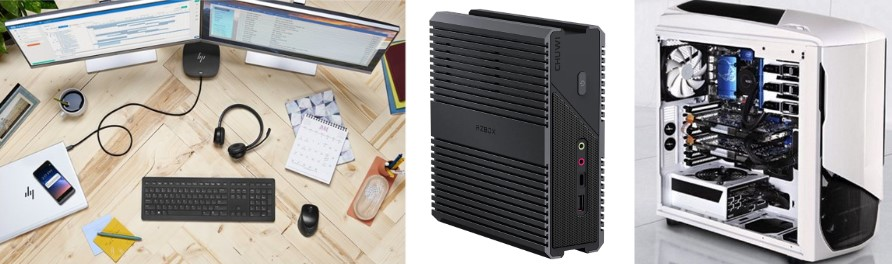
\includegraphics[width=1\textwidth]{./figuras/laptop_minipc_torre.jpg}
\caption{Portátil, mini pc y torre, google images. }
\label{F:laptop_minipc_torre}
\end{center}
\end{figure}

Por último tenemos los mini-pc o torres-slim, contienen un hardware potente para uso 'adecuado', poco actualizable pero muy asequible, además de un volumen reducido y la posibilidad de ser reubicado fácilmente, sin tener la autonomía de un laptop.

Ante un presupuesto fijado a 6-8 años vista, se pueden emplear dos estrategias, 'hardware potente mantenido', o el uso de 'hardware medio pero reemplazable' a 3-4 años, siendo presupuestaria mente equivalentes.

Como recomendación de este autor adoptó ampliamente del uso portátil como elemento más interdisciplinar, autónomo y de fácil uso. Sin embargo para aquellas startups o oficinas físicas el uso de mini-pc puede ser un nicho muy interesante. La estrategia de reemplazo dependen de las circunstancias tecnológicas del mercado en el momento de la compra que son explicadas en los apartados de CPU y RAM.

\subsection{Pantalla, comodidad y opinión}\label{S:pantallas}
Tenemos 'el dilema del tamaño, forma y número de pantallas'; no existe un consenso claro, excepto de que es necesario 1 o más monitorios para trabajar “adecuadamente”, es decir, la pantalla del laptop más un monitor extendido; una gran pantalla o dos pantallas en caso de pc o mini-pc. 

Existe un gran debate sobre si la disposición de los monitores debe ser 16:9 en tamaño de 21’-24’/27’ o de 21:9 en 30’-34’ pulgadas. Mi punto de vista es:  dos pantallas en caso de pc; depende del espacio, presupuesto y tamaño en el caso de laptop.

\begin{figure}[!htb]
\begin{center}
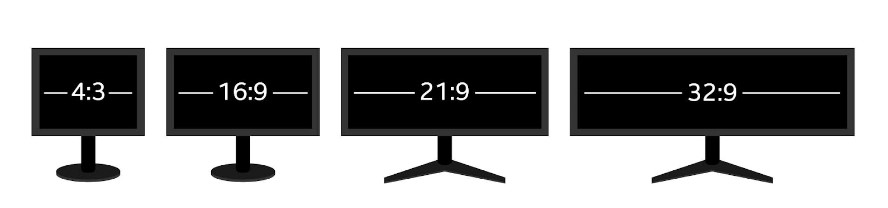
\includegraphics[width=1\textwidth]{./figuras/pantallas_geometria.jpg}
\caption{Monitores, formas y geometrías \cite{i_pantallas}. }
\label{F:pantallas_geometria}
\end{center}
\end{figure}

En mi opinión, si el portátil es “versátil” en movilidad, no supera las 13’-15’ por lo que requiere dos pantallas como un pc, de 24’ o 27’ ambas con las mismas características. Si el portátil tiene una pantalla “adecuada” para trabajar 16’-17’, puede elegir una única pantalla extendida, siendo recomendable 30’-34’ disposición 21:9.

La realidad es que si el presupuesto y el espacio lo permite, he llegado a ver el uso de 3 y 4 pantallas obviando la propia del portátil.

Requisitos indispensables son la resolución mínima FHD (1920x1080), adecuada QHD (2K) y óptima UHD (4k) , tecnologías “eye care” y una frecuencia alta 60-75 hz (adecuado) para reducir el esfuerzo visual. Cualquier otro detalle fuera de estos queda catalogado como customización en función del precio-calidad, ya que mejoras sensibles en las pantallas con un gran presupuesto pueden quedar totalmente degradadas con una inadecuada iluminación ambiental.

\begin{figure}[!htb]
\begin{center}
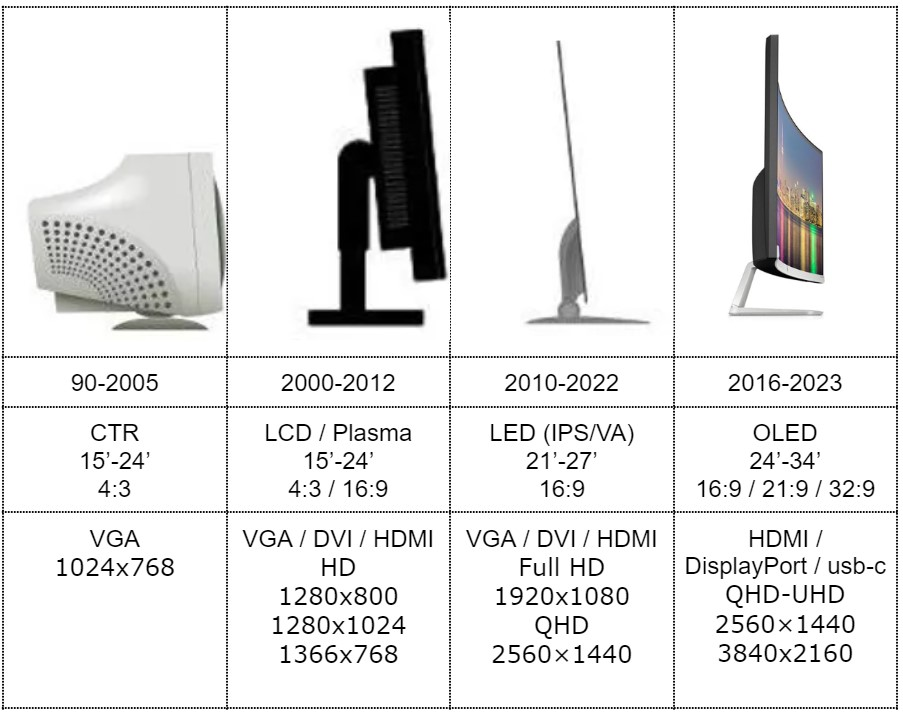
\includegraphics[width=1\textwidth]{./figuras/comparacion_monitor_tech.jpg}
\caption{ Evolución tecnológica monitores ultimos 30 años.}
\label{F:comparacion_monitor_tech}
\end{center}
\end{figure}

Importante resaltar (véase fig. \ref{F:comparacion_monitor_tech}) que el mundo de los monitores, evoluciona más lentamente en una perspectiva 5-10 años, donde la vida media de una pantalla excede los 12 años, por lo que suelen reemplazarse tecnológicamente cuando superan los 10 años por calidad en relación a sus prestaciones-precio.

Por lo tanto no es una cuestión de requisitos mínimos, sino de una tendencia económica, donde a un rango de precio “profesional” evoluciona con mejoras técnicas (resolución, tecnología, espacio-forma) a un precio equivalente. Como dato re-marcable\cite{c_resolucion_estadisticas_W3Schools} las pantallas más compradas en 2020-22 fueron 24’, 27’, 32’ con resolución FullHD, así como la resolución más utilizada en webs de programadores fueron 40\% superiores Full HD, 20\% Full HD y 30\% inferiores.

Como conclusión entenderemos que \textbf{no tiene sentido reemplazar los monitores con menos de 5 años}, así como \textbf{suele ser práctico-económico a partir de los 8 años}, pero se puede trabajar adecuadamente con ellos hasta el final de su vida útil 12 años, que es lo que reflejan las estadísticas de resolución utilizada en navegadores.

\subsection{Hardware y recursos}\label{S:hardware_recursos}
El hardware y recursos empleados evolucionan en el tiempo (a una velocidad más rápida que los monitores), la vida media de un setup actual es de \textbf{4-6 años}, no superando los 8 años, durante los cuales es necesario un mínimo de actualizaciones, mantenimiento o reemplazo de piezas. Así mismo la usabilidad se resiente especialmente en baterías o equipos sin el apropiado mantenimiento.

Actualmente la gran mayoría de PC de 2010-2013 aún están en funcionamiento, 10 años después, algo verdaderamente improbable en los años 80 's, 90' s,  o principios de 2000.

 La realidad es que se ha ganado en rapidez y cantidad pero especialmente en multitasking, especialmente en programas de grandes volúmenes de datos, es decir, ‘más cantidad que calidad’. Por lo que los requisitos tanto del sistema operativo como de los programas más comunes son ampliamente movidos por hardware viejo. Por otro lado, el espacio en disco o la velocidad de acceso, así como la memoria RAM evolucionan continuamente aumentando velocidades y capacidades a un coste inferior, lo cual ha permitido mejorar los cuellos de botella en aquellos hardwares viejos con actualizaciones sencillas véase \cite{c_guia_hardware}. Este punto debe aclararnos que el mantenimiento es un elemento muy critico, especialmente si esperamos extender la vida del hardware 8-12 años para otras tareas no profesionales.

 \subsection{Periféricos}
 Entendemos como periféricos aquellos elementos externos que usualmente se conectan por USB o bluetooth. Un hub de conectividad o hub de monitor externo es obligatorio, así como se sobreentiende un ratón y teclado. Existen varios elementos dignos de mencionar en la catalogación de los mismos:
 \begin{itemize}
     \item Auriculares y uso del micrófono-cámara del portátil (mínimo). Auriculares de alta calidad con micrófono (adecuado), auriculares con cancelación de ruido y micrófonos HD (óptimo), web-cam HD con micrófono con cancelación de ruidos (óptimo).
     \item Plataforma de elevación laptop (adecuado), plataforma hub con refrigeración activa laptop (óptimo).
     \item Sistemas de autenticación externos, lector de huellas, lector de tarjeta etc…. (óptimo).
     \item Panel táctil y bolígrafo asociado (óptimo), pantalla táctiles asociada a monitor o laptop (óptimo).
     \item Google home, Alexa, u otros elementos de domótica, automatización, fuentes musicales o notificaciones. (óptimo, pero requiere de análisis riesgos de seguridad).

     \item Requerimientos especiales, impresora-scaner, impresoras 3d, electrónica de monitorización o placas prototipado. (solo bajo necesidad práctica).
 \end{itemize}

  \subsection{Gestión del setup}
  Existe una norma bastante compleja ya que la gestiona cada individuo, cuyo objetivo es separar el trabajo de tu vida personal. En muchos casos aunque un despacho o habitación dedicada a tu setup sirve como jaula de aislamientos y concentración. La realidad es que gran cantidad de profesionales tiene intereses alineados o coincidentes con sus labores profesionales y de igual manera tiene sus necesidades personales de acceso a la información, cuentas personales, almacenamientos, documentos y juegos.

¿Cómo separar el pc personal del profesional?

Un buen profesional no debe usar su setup profesional para usos personales, primero para mantener esta estricta separación que no afecte o predisponga a distracciones de índole personal durante la jornada laboral. Por otra parte están los riesgos de ciber seguridad de generar un agujero de seguridad desde sus cuentas personales a sus servicios profesionales.

\subsubsection{Aislamiento de navegación}
La gran mayoría de servicios personales a día de hoy son capaces de ser usados vía navegador, así como el acceso a noticias, comunicaciones en línea y servicios streaming como pueden ser música. La primera capa de seguridad es separar y la gestión de nuestras cuentas personales y profesionales en diferentes cuentas de sincronización. Permitiendo acceder a dos cuentas vía nuestro navegador, y evitando almacenar contraseñas, historial de navegación, cookies y otros elementos. Una separación más estable es el uso de diferentes navegadores para cada una de las cuentas, así evitamos una gestión compleja o la afectación de plugins inseguros en el navegador.

En mi opinión son una buena opción, aunque solo debe usarse en momentos de necesidad y debe evitarse lo máximo posible.

La opción más adecuada para dichos casos tales como revisar mails, esperar un mensaje vía whatsapp o simplemente poner tu playlist de relajación en los altavoces pasa por el uso de \textbf{un 2º elemento personal móvil/tablet/laptop} capaz de surtir dicha función sin necesidad de usar tu hardware profesional e \textbf{incluso utilizando diferentes redes} para conectarse.

\subsubsection{Setup Conmutable}
Sin embargo qué hacemos cuando en la post jornada laboral deseo trabajar en mi hobby tecnológico, o simplemente jugar o ver series desde mi pc personal.¿Debo acaso duplicar recursos teniendo un precioso despacho con un setup con múltiples pantallas?

La respuesta es simple; \textbf{No}. Si seleccionamos adecuadamente los monitores a elegir, así como el dock-station o hub de periféricos, pronto entenderemos que es fácil disponer de hasta 3 o 4 fuentes de imagen independientes, múltiples fuentes de sonido y un uso compartido de periféricos. 

\begin{figure}[!htb]
\begin{center}
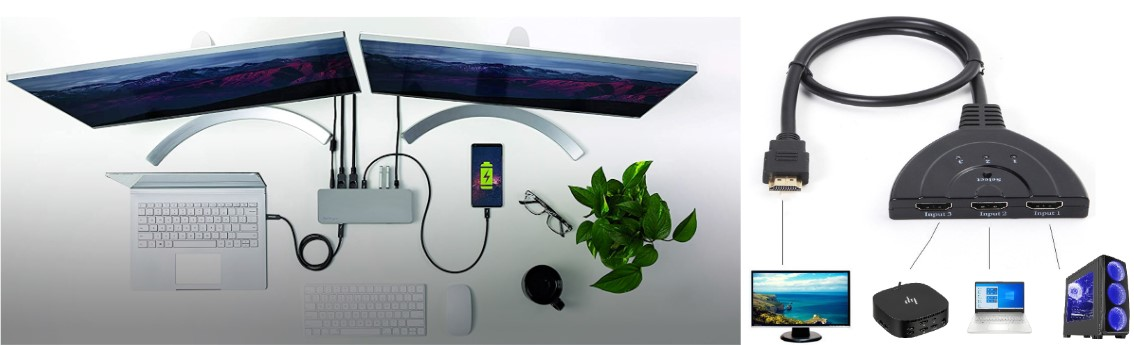
\includegraphics[width=1\textwidth]{./figuras/conectividad_monitores.jpg}
\caption{ Conectividad de monitores, amazon products.}
\label{F:conectividad_monitores}
\end{center}
\end{figure}

Se puede optar por la estrategia centralista, todo se conecta a nuestro hub y con conmutar la conexión usb hub-portátil de laptop profesional a personal ya tenemos el setup completo para uso personal. O se puede seguir una estrategia de fuentes en paralelo, de tal manera que ambos hardware están conectados a puertos diferentes o a través de un multiplexor. Si solo uno está encendido, basta con cambiar de pc/laptop el usb que controla el teclado-ratón o el hub de usb y ya podemos utilizar el setup. Si ambos están encendido, requiere seleccionar en las pantallas la fuente a mostrar y conectar el teclado-ratón aquel que queramos usar.

En mi opinión la segunda opción es más interesante aunque compleja, requiere de una mayor planificación, pero facilita la simultaneidad de 3 o 4 pc, pudiendo estar conectado en sesiones en remoto desde aquel que gestione las pantallas.

\section{Abastecimientos auxiliares}\label{S:abastecimientos_auxiliares}
Abastecimiento auxiliares, son todas aquellas infraestructuras o herramientas necesarias para poder usar nuestro setup adecuadamente. Entre las principales necesidades tenemos los suministros de electricidad, climatización y acceso a internet. Otros interesantes son aquellos que usamos como alternativa funcional cuando un suministro básico falla, sistemas de alimentación ininterrumpida (SAI) o equivalentes, acceso alternativo a la red, setup mínimo alternativo o una planificación aceptable en caso de NO poder realizar home office. 

\subsection{Suministro Eléctrico}
Este elemento parece simple y obviamente necesario, pero a parte de la disponibilidad de red eléctrica y de la partida compensatoria en el acuerdo de teletrabajo qué implicaciones tiene en nuestro oficina el suministro eléctrico.

Disponibilidad de enchufes o switch, verdaderamente es complejo alimentar 2 pantallas, un hub, un portátil, una lámpara y algún que otro periférico extra. Aun lo es más si el sistema eléctrico es viejo y el único enchufe disponible tiene una amalgama de extensores-ladrones interconectados entre ellos. Recordemos que los enchufes tradicionales tienen 10-16A como límite, así como muchos 'alargos' no utilizan cable de 2.5 $mm^{2}$ sino 1.5 $mm^{2}$ de sección.

\begin{figure}[!htb]
\begin{center}
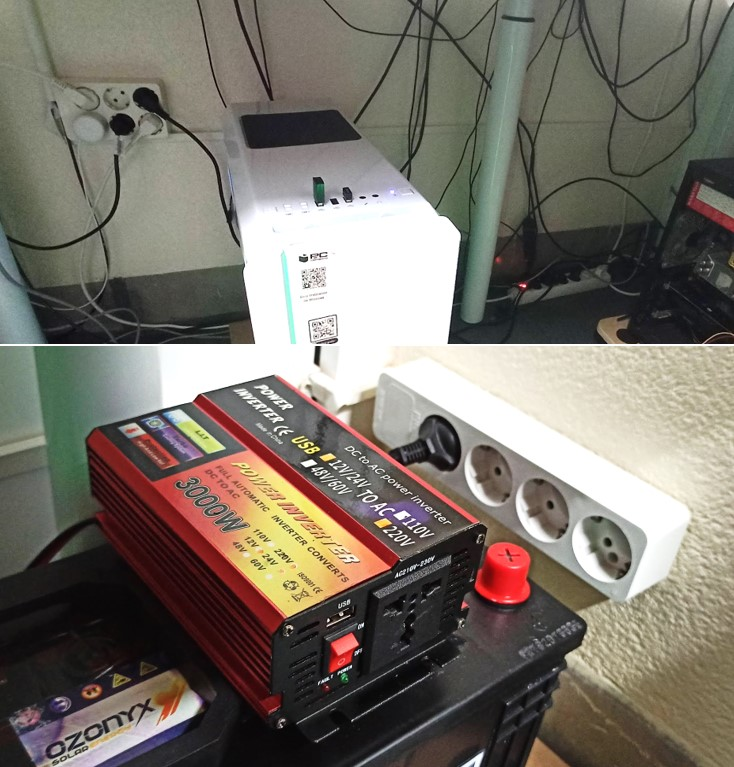
\includegraphics[width=0.75\textwidth]{./figuras/instalacion_electrica.jpg}
\caption{ Enchufes e instalación eléctrica.}
\label{F:instalacion_electrica}
\end{center}
\end{figure}

Como conclusión hemos de recordar que si bien un setup no es una actividad industrial requerirá de un mínimo de 6 enchufes-switch y raramente supera un consumo límite de una toma en torno a los 2000-2500W pero si puede ser un problema en una oficina de una startup afincada en un antiguo piso, especialmente cuando se usan elementos como calefactores o múltiples estaciones de trabajo no planificadas previamente. En dicho caso recomendamos no solo la instalación de múltiples switches con el cableado adecuado, sino el aislamiento de las filas o islas de trabajo, en PIAs\cite{c_pia} independientes con el fin de aislar y detectar fallos eléctricos que no afecten a la oficina de manera generalizada.

\subsection{Climatización}
Este punto tiene controversia entre oficinas como en gastos de teletrabajo. En mi opinión, la temperatura de trabajo óptima es un tema muy personal, sin embargo se recomienda entre 23º-27º en verano y 17º-24º en invierno. El verdadero punto importante es la existencia de una ventilación continuada y adecuada que reduzca los riesgos contaminantes, alérgenos y degradación de la calidad del aire.

Vivo en una zona privilegiada “Costa Daurada” de Tarragona cuyo invierno no baja de los 8º-10º y las temperaturas veraniegas raramente superan los 38º. Por lo que con apenas el aislamiento de la vivienda y una adecuada ventilación bien puede entrar dentro del intervalo de confianza de manera pasiva. Sin embargo nadie ha hablado de la humedad, la cual en la costa es siempre superior al 60\% (invierno) y mayor al 90-95\% (verano).

A su vez, un trabajo en remoto significa, poco movimiento físico y contacto continuado de extremidades con silla y escritorio, por lo que por experiencia propia puedo decir que no se puede trabajar adecuadamente con más de 28º en verano, ni menos de 18º en invierno, sea cual sea la ropa utilizada debido a la alta humedad ambiente y la naturaleza del trabajo.

Como conclusión los ventiladores o calefactores eléctricos son “mínimos”, un spliter de bomba calor frío “adecuado”, usar la aclimatación general de la casa “óptimo” pero costoso. En la instalación de la caseta se opto por un pingüino (bomba de calor/frió), sin embargo se ha desmantelado y sustituido vease mejoras de 2023 \ref{S:cambios_bombacalor}.

\subsection{Acceso a Internet}
Los requisitos de acceso a la red son un elemento crítico para el home office, no solo por las características necesarias sino porque dicho medio es compartido en la vivienda por los usos particulares de la familia. 
\begin{figure}[!htb]
\begin{center}
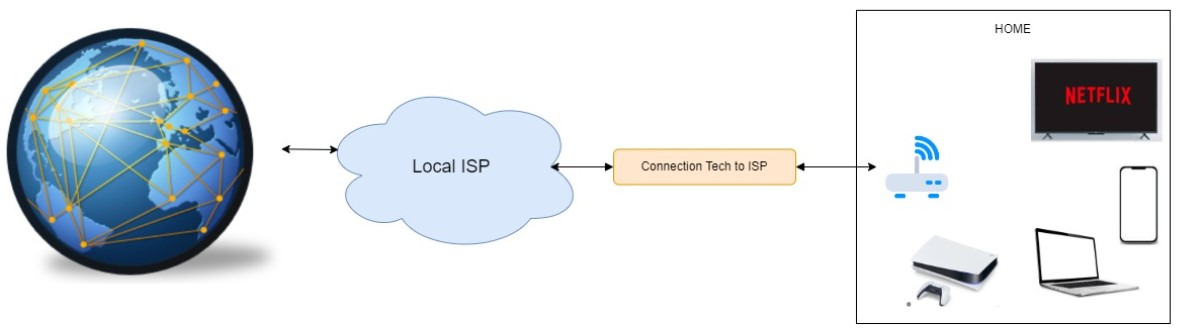
\includegraphics[width=1\textwidth]{./figuras/conexion.jpg}
\caption{Diagrama de conexión. }
\label{F:conexion}
\end{center}
\end{figure}
Por lo tanto la “velocidad” de la conexión debe permitir establecer videoconferencias junto al uso de streaming (netflix,spotify…) u otros usos personales de alta demanda. En la implementación física de mi oficina, usamos mi conexión familiar de 600 Mbps de fibra simétricos que escede ampliamente las necesidades.

\subsubsection{Ancho de banda}
Ancho de banda (BW), tasa o velocidad es la capacidad de transmisión de datos por segundo que permite la conexión de manera estable e ininterrumpidamente. Existen conexiones simétricas, velocidad de subida (uplink) y bajada (downlink) idénticas, y asimétrica donde la uplink suele ser inferior (entorno a un 20-30\% del downlink).

Una vídeo conferencia exigente, con múltiples usuarios enviando imagen y sonido HD con posibilidad de pantalla compartida, requiere de un mínimo de 4-8 Mbps. Una transmisión HD en netflix oscila entre 3-5 Mbps, 15 Mbps si es 4K. Se sobre entiende que en un contexto de coexistencia familiar y de posible ejecución en paralelo de más actividades profesionales, un uso mínimo  requiere una conexión de 10/3 Mbps (uplink/downlink), una conexión adecuada \textbf{15/5 Mbps} y una óptima son aquellas con tasas superiores a los 20/10 Mbps.

El ancho de banda de una conexión está intrínsecamente definido por la tecnología de acceso proveída por el ISP local, ejemplo conexión fibra movistar 100/100 Mbps. Pero influenciado por la congestión del ISP local o nodos intermedios, como ejemplo de las 100 megas simétricas, mi conectividad con diferentes servidores españoles puede ser de 60-80 Mbps (inferior a la conectividad directa con el ISP) y usualmente asimétrica, pero podemos obtener medidas de 15-30 Mbps con servidores asiáticos.

\subsubsection{Latencias}
La latencia, coloquialmente llamada lag o ping, es el tiempo medio de ida o vuelta en una conexión de red, es decir el tiempo mínimo de interacción entre dos elementos de la red. 

Las personas detectamos que la comunicación no es “instantánea”, si la interacción de dos interlocutores es superior a los 300 ms (1/3 segundo), por lo que en telefonía se establece un umbral de 150 ms como latencia máxima a partir de los cuales se percibe una comunicación deficiente, las diferentes plataformas de videoconferencias marcan como deficiente una conexión con ping superiores a 100 ms. Por lo tanto latencias 100-150 ms (mínimo), \textbf{50-100 ms (adecuado)}, inferiores a 50 ms óptimo.

Se ha de resaltar que el tipo de tecnología usada entre la oficina y el ISP (red de acceso) puede suponer el 60\% de la latencia a excepción de la fibra. Pero además aquellas conexiones con más nodos intermedios, es decir, normalmente más lejanas geográficamente acumularan una mayor latencia, debido a la red de transporte. 

\subsubsection{Jitter}
Jitter o fluctuación de retardo es la variabilidad temporal del retardo. Conceptualmente podemos entender que si la latencia es el valor medio, la medición del jitter puede realizarse de diversas maneras como aquellos retardos máximos o usualmente estadísticos como la desviación típica de la latencia.

La principal consecuencia en comunicación online es que aunque la latencia media es aceptable, puede que un 20-30\% de los paquetes tengan retardos mayores o desiguales.

Aunque puede solucionarse con estrategias de buffer, en videoconferencia los buffer tienen tamaños de 50ms, implica la pérdida de información y por ende cortes o inteligibilidad de la comunicación. Por lo tanto jitter max 40 ms requisito mínimo, \textbf{inferior a 30 ms adecuado}, inferior a 10 ms óptimo.

\subsubsection{Tecnologías aptas}
\definecolor{naranja}{rgb}{1.0, 0.49, 0.0}
A la hora de analizar las diversas tecnologías de acceso a internet, las evaluaremos desde el punto de vista “adecuado” (\textcolor[cmyk]{1,0,1,0}{verde}), azul (\textcolor{blue}{óptimo}), aquellas conexiones insuficientes (\textcolor{naranja}{naranja}) para adecuado y aquellas conexiones que no cumplen los requisitos mínimos(\textcolor{red}{rojo}). 

\begin{table}[htb]
    \centering
    \label{T:comp_conexion_tech}
    \caption{Comparación Tecnológias de acceso}
    \begin{tabular}{|p{2.5cm}|p{2cm}|p{2cm}|p{1.75cm}|p{1.75cm}|p{2cm}|}
    \hline \hline 
        ~ & \textbf{Velocidad Downlink} & \textbf{Velocidad Uplink}  & \textbf{Latencia} & \textbf{Jitter} & \textbf{Coste} \\ \hline
        \textbf{Requisitos Adecuados} & \textbf{15 Mbps}  & \textbf{5 Mbps}  & \textbf{75 ms } & \textbf{30 ms}  & \textbf{Profesional}  \\ \hline
        \textcolor{red}{ADSL/ADSL2 (zona alejada)}\cite{c_dsl_tech}  & \textcolor{red}{6-8 Mbps}  & \textcolor{red}{1-2 Mbps}  & \textcolor{naranja}{50-90 ms}  & 15-25 ms  & Básico  \\ \hline
        \textcolor[cmyk]{1,0,1,0}{ADSL/ADSL2+ (zona céntrica) }\cite{c_dsl_tech}  & 16-22 Mbps  & 4-6 Mbps  & 30-60 ms  & 15-20 ms  & Profesional  \\ \hline
        \textcolor[cmyk]{1,0,1,0}{VDSL2 (zona céntrica) }\cite{c_dsl_tech}  & 15-50 Mbps  & 5-18 Mbps  & 15-50 ms  & 10-20 ms  & Profesional  \\ \hline
        \textcolor[cmyk]{1,0,1,0}{Coaxial/cable}  & 30-300 Mbps  & 3-30 Mbps  & 10-30 ms  & 10-15 ms  & Profesional  \\ \hline
        \textcolor{naranja}{3G/4G}  & \textcolor{naranja}{10-80 Mbps}  & 5-30 Mbps  & \textcolor{naranja}{20-80 ms}  & 15-30 ms  & Profesional Pro  \\ \hline
        \textcolor{naranja}{WIMAX Otros Radio link}\cite{c_wimax_tech}  & \textcolor{naranja}{6-30 Mbps}  & \textcolor{red}{1-3 Mbps}  & \textcolor{naranja}{30-80 ms}  & \textcolor{naranja}{15-40 ms}  & Profesional Pro  \\ \hline
        \textcolor{red}{Satellite Link (traditional GEO)} & 10-50 Mbps  & \textcolor{naranja}{1-6 Mbps}  & \textcolor{red}{500-800 ms}  & \textcolor{naranja}{20-50 ms}  & Profesional Pro (Spain*)  \\ \hline
        \textcolor{red}{Satellite Link (LEO )}  & \textcolor{red}{1-10 Mbps}  & \textcolor{red}{0.5-2 Mbps}  & \textcolor{naranja}{50-150 ms}  & \textcolor{naranja}{20-40 ms}  & Profesional Pro  \\ \hline
        \textcolor{blue}{StarLink}\cite{c_starlink_tech}  & 100-400 Mbps  & 5-50 Mbps  & 15-50 ms  & 10-40 ms  & Business  \\ \hline
        \textcolor{blue}{Fibra Básica}  & 50-100 Mbps  & 10-50 Mbps  & 5-15 ms  & 5-10 ms  & Básico-Profesional  \\ \hline
        \textcolor{blue}{Fibra}  & 300 Mbps - 1 Gbps  & 100 Mbps - 1 Gbps   & 1-15 ms  & 1-10 ms  & Profesional Pro  \\ \hline
    \end{tabular}
\end{table}

Se ha de destacar que desde el punto de vista práctico calidad-precio, las mejores opciones son \textbf{la fibra básica, conexión coaxial o VDSL+ \cite{c_dsl_tech} en zona céntrica}.

Aquellas conexiones que dependen de enlaces radio (naranja), cumplen los requisitos, pero tienen valores inferiores o degradados en aquellas áreas geográficamente problemáticas, las cuales no tienen la posibilidad de otro tipo de conexión.

Una vez tenemos una conexión adecuada, en muchos casos el factor limitante no es el tipo de conexión sino el medio de transmisión en la propia vivienda. Las tecnologías más utilizadas son WIFI, PLC\cite{c_plc_tech} y cableado.

\textbf{Obviamente cableado es la mejor opción }permitiendo 1-2.5 Gbps, robusto a interferencias, y no afectado por el número de elementos en la red, así como físicamente ciber- seguro.
Los PLC, permiten velocidades de 10-500/5-50 Mbps no aumentando significativamente la latencia ni el jitter, por lo que son una alternativa mejor que los medios inalámbricos en muchos casos.

El uso de Wifi y repetidores depende tanto de la vivienda, materiales así como elementos conectados. Es de especial interés entender que cuanto mayor sea el número de elementos conectados, o repetidores, menor será la velocidad efectiva de acceso al medio puesto que este es compartido. Es un medio inalámbrico sensible a interferencias y comparte canales con vecinos-geográficos que interfieren la señal. Por otra parte incrementa sensiblemente tanto latencias pero especialmente Jitter, tiene pérdidas más significativas que los medios físicos no inalámbricos.

Así mismo se debe comprender que la velocidad media será afectada por el elemento más lento (más alejado y con estándar más antiguo). Por lo tanto se recomienda la coexistencia de viejos y nuevos estándares con la finalidad de que aquellos elementos de estándares b/g/n se conecten a un AP diferente de los ac/ax. Así como una separación del AP-profesional del AP-familiar. Por último es interesante evaluar si definir canales estáticos, minimizando la interferencia externa y usando canales diferentes en nuestros AP, o el uso de algoritmo de asignación automática.

Conclusión el wifi es aquel elemento que puede tener un rango tan ambiguo de aplicaciones y casuísticas que aun permitiendo en algunos casos mejores performance que cableado (wifi 6 802.11.ax) y siendo la instalación más ágil y sencilla, no es la recomendación de este trabajo. Se recomienda el cableado o uso de PLC  como conexión preferente, con opción a la instalación de un punto wifi en la localización del Setup para uso exclusivo profesional (separación de redes).

\subsubsection{StarLink o el 5G}
La principal característica de las nuevas tecnologías de comunicación inalámbricas se basa no solo en un aumento significativo de la velocidad de transmisión sino de una reducción drástica de las latencias en la red troncal del operador de telecomunicaciones.

Por ello el 5G, su principal virtud no es la alta velocidad sino la baja latencia y jitter, así como la movilidad urbana que permite.

De una manera muy similar Starlink permite la comunicación directa de su red satélital de órbita baja mediante láseres. La reducción de las distancias respecto a satélites en órbitas más altas, así como su cobertura global y facilidad de conmutado en su red esférica, permite obtener bajas latencias inferiores a las conexiones físicas por fibra entre puntos muy distantes en el mundo y una disponibilidad de cobertura completa con excepción de las regiones polares.

Estos puntos pueden ser de interés para actividades estratégicas, fast-trading mundial, seguridad e independencia política de la conexión, o un modo de vida nómada, como puede ser un freelance que vive-trabaja en una casa-barco, moviéndose por diferentes regiones, pero totalmente descartable para el 99\% de los casos de uso común en España, especialmente debido a su \textbf{coste business}.

\subsection{Circunstancias e histórico}\label{S:circunstancias}
Desde 2014 en mi etapa de becario me he dedicado a tareas concretas de ingeniería entremezcladas con la automatización y la programación desde algorítmica básica, programas de gestión. Así mismo desde 2016  me he dedicado a programación, especialmente backend de manera profesional en frameworks de php, python y java.

En 2018 me mudé a un barrio residencial baix penedes que es desde entonces mi actual residencia. El lugar puede describirse como el perfecto barrio residencial, a menos de 1 km de la playa, en una zona muy tranquila zona ampliamente turística y llena de segundas residencias dentro del límite del área metropolitana de Barcelona.

Un punto importante de esta localización, es la pésima infraestructura tecnológica e incluso infraestructura eléctrica de las costas del Baix Penedes. Históricamente la nula planificación, la rápida y exponencial urbanización durante el boom inmobiliarios del último lustro, junto a una infraestructura no dimensionada correctamente para las fluctuaciones de la temporada turística concluye en las siguientes casuísticas:
\begin{itemize}
    \item Apagones, fluctuaciones de corriente o problemas variados durante las temporada turística (junio-septiembre) y navidades, problemas eléctricos relacionados con inundaciones en otoño. Que pueden dejar la zona durante intervalos de 2-3 horas varios días ante una incidencia y su resolución.
    \item Nula conectividad por cobre o fibra, únicamente proveedores de WIMAX\cite{c_wimax_tech} o wifi por antenas point to point y conectividades inferiores a 5 Mbps en cableado antiguo de cobre. Completamente deficientes bajo condiciones meteorológicas adversas y afectadas por picos de demanda.
\end{itemize}

\subsubsection{Pre pandemia}
Se disponía de una habitación de estudio para mi etapa estudiantil de máster, hobbies o zona de estudio/trabajo compartido con mi pareja.
\begin{figure}[!htb]
\begin{center}
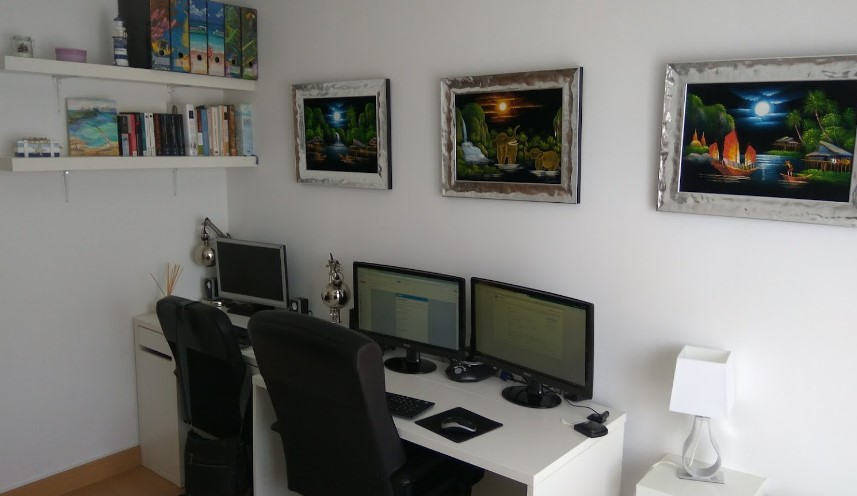
\includegraphics[width=0.8\textwidth]{./figuras/setup_cero.jpg}
\caption{Setup pre pandemia.}
\label{F:setup_cero}
\end{center}
\end{figure}

Curiosamente pocos meses antes de la pandemia, con el objetivo de cumplir la cobertura 90\% establecida por ley para 2020\cite{c_boe_fibra}, se desplegó satisfactoriamente una red de fibra en toda la zona residencial, permitiendo conectividades simétricas de hasta 300 Mbps.

Afortunadamente en mis planes familiares ya contaba con una reforma y mejora de la sala de estudio para adecuarla como dormitorio con escritorio, pudiendo usar como zona de trabajo o habitación de invitados, en perspectiva a un futuro familiar como habitación para un niño o niña.

\begin{table}[htb]
    \centering
    \caption{Setup pre pandemia tabla comparativa}
    \label{T:comp_setup_prepandemia}
    \begin{tabular}{|p{2.5cm}|p{2.5cm}|p{2.5cm}|p{2.5cm}|p{2.5cm}|}
    \hline   \hline
        ~ & \textbf{Zona de trabajo} & \textbf{Hardware} & \textbf{Red} & \textbf{Otros} \\ \hline
        \textbf{Setup} & Escritorio dedicado Sillas de estudio & 2 pantallas 21’ HD PC old-2011 laptop 2013 & Wimax 2/3Mbps Wifi g 54 Mbps & Iluminación  natural y artificial adecuadas \\ \hline
       \textbf{Defectos o planes pendientes} & Mesa baja y poco ancha & Viejo, uso hobbies & Mejora a Fibra pendiente  & Mayor capacidad de almacenaje y eliminación de 2º escritorio diminuto  \\ \hline
    \end{tabular}
\end{table}

 Desde la llegada de la fibra también realice las incorporaciones de una pizarra y una impresora 3D para mis hobbies, así como un cableado de la habitación con ethernet para obtener la máxima velocidad y no ocupar la red Wifi.

 \subsubsection{Pandemia}\label{S:setup_pandemia}
 Dos semanas antes de los reales decretos que pusieron en marcha los mecanismos de aislamiento de la pandemia, la empresa en la que trabajo me proporcionó un portátil como nuevo hardware de trabajo, las credenciales y una vpn para conectarme, comenzando inmediatamente el 100\% del trabajo en remoto como medida precautoria.
 
\begin{figure}[!htb]
\begin{center}
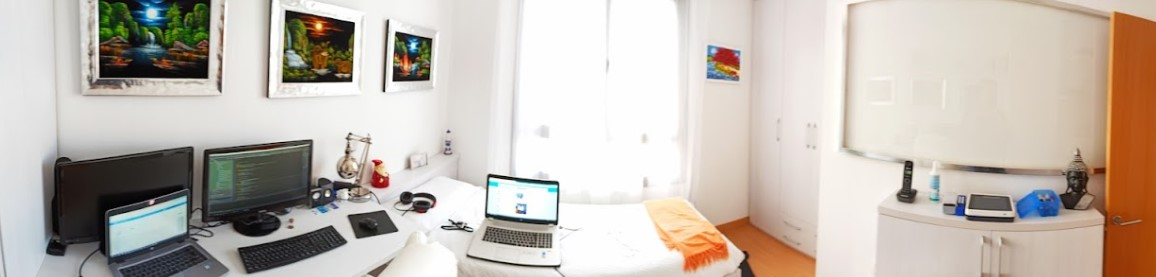
\includegraphics[width=0.95\textwidth]{./figuras/setup_uno.jpg}
\caption{Setup pandemia.}
\label{F:setup_uno}
\end{center}
\end{figure}

Los recientes cambios en la habitación de estudio me permitieron un teletrabajo satisfactorio únicamente degradado por pequeños problemas fácilmente solucionables como la adquisición de un split usb-vga para la utilización de ambos monitores con el portátil laboral, junto a la conexión de mi pc personal.

\begin{figure}[htb]
\begin{center}
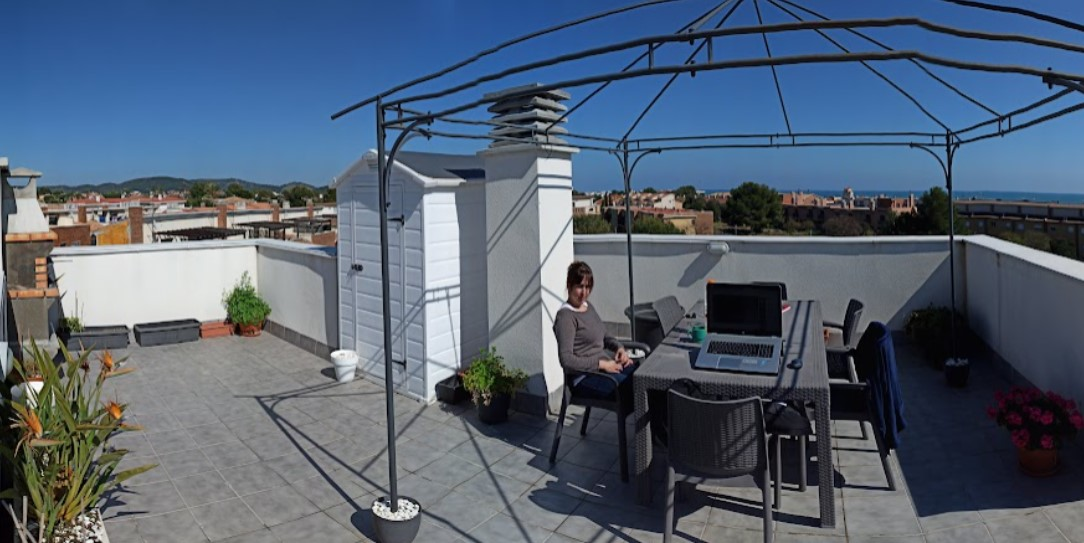
\includegraphics[width=0.9\textwidth]{./figuras/terraza_cero.jpg}
\caption{Terraza en pandemia.}
\label{F:terraza_cero}
\end{center}
\end{figure}

Una de mis tareas de bricolaje durante la pandemia fue la mejora con la instalación de cableado eléctrico para iluminación y enchufes en la terraza. Incluyendo red eléctrica en una caseta de almacenaje situada en la misma. 

\begin{table}[htb]
    \centering
    \caption{Setup Pandemia tabla comparativa}
    \label{T:comp_setup_pandemia}
    \begin{tabular}{|p{2cm}|p{3cm}|p{2.75cm}|p{2.75cm}|p{2.75cm}|}
    \hline   \hline
        ~ & \textbf{Zona de trabajo} & \textbf{Hardware} & \textbf{Red} & \textbf{Otros} \\ \hline
        \textbf{Setup incremental} & +Zona de trabajo a medida adecuada +Mesa alta (+70cm) +Mueble a medida con pc, cableados ocultos +gran capacidad organizativa y de almacenamientos +impresora 3D oculta en armario & +incorporación de split usb en pantallas +cam HD +micro-auricular HD +switch ethernet & +Fibra 300Mbps +Wifi n 150 Mbps / 5G 300 Mbps + cableado ethernet & +Pizarra translúcida +cableado interior de la casa con ethernet + impresora 3D y otros elementos \\ \hline
        \textbf{Defectos o planes pendientes} & Perfecta, pero habitación planificada invitados y futuros hijos.  & Pantallas deficientes Hardware viejo & Ethernet a 100 Mbps mejorable a giga ethernet & La climatización e infraestructuras dependen de la casa. \\ \hline
    \end{tabular}
\end{table}

Con el objetivo de poder disfrutar de horas de luz y la salida al exterior en los continuados confinamientos, instale un PLC\cite{c_plc_tech} que permitía una conectividad de 7-12 Mbps emitiendo una señal wifi en la caseta de la terraza. Permitiendo trabajar algunas horas especialmente por la tarde cuando la intensidad lumínica no deslumbraba la pantalla.

Durante el año 2020, quedó patente la funcionalidad plena de la habitación de estudio como habitación dedicada a teletrabajo, reflejando aquellos punto mejorables, sin embargo también quedó patente la infraestructura del barrio, tiene 3-4 días anuales con incidencias eléctricas cuando el calor o el frío sobrecarga la infraestructura, requiriendo de un plan “b” para dichos días.

Este periodo lo damos por concluido tras finalizar los períodos de aislamiento excepcionales en 2021 y las campañas de vacunación. El teletrabajo 100\% fue continuado como medida precautoria hasta 2023.

\subsubsection{Post pandemia}
Finalmente la mayoría de los puntos mejorables como las pantallas, uso de silla ergonómica-gamer y diversos periféricos o hub fueron subsanados.

\begin{figure}[!htb]
\begin{center}
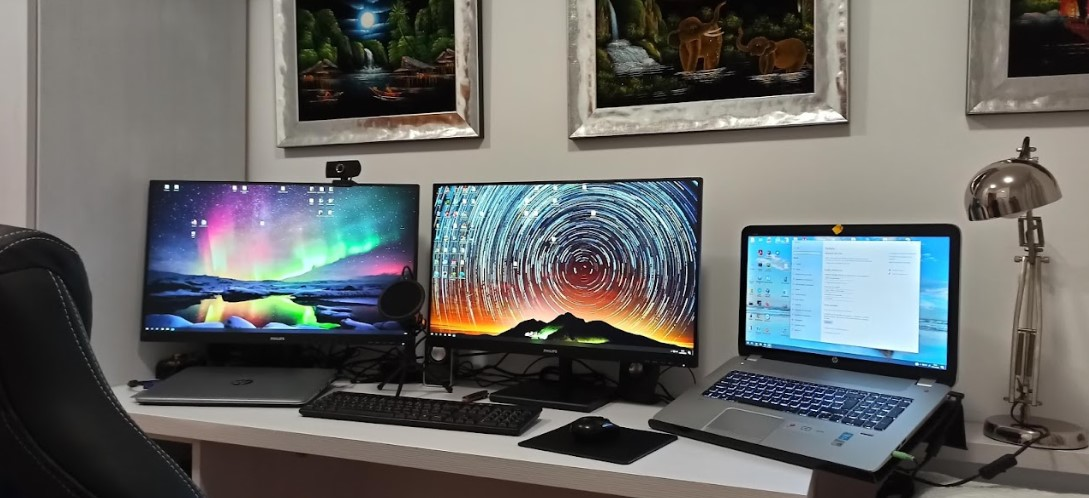
\includegraphics[width=0.85\textwidth]{./figuras/setup_dos.jpg}
\caption{Setup post pandemia.}
\label{F:setup_dos}
\end{center}
\end{figure}

Sin embargo, desde el verano de 2021, quedó patente que el principal problema era la “planificación familiar”, básicamente esa habitación estaba destinada a habitación de niño/niña con escritorio propio.
\begin{figure}[htb]
\begin{center}
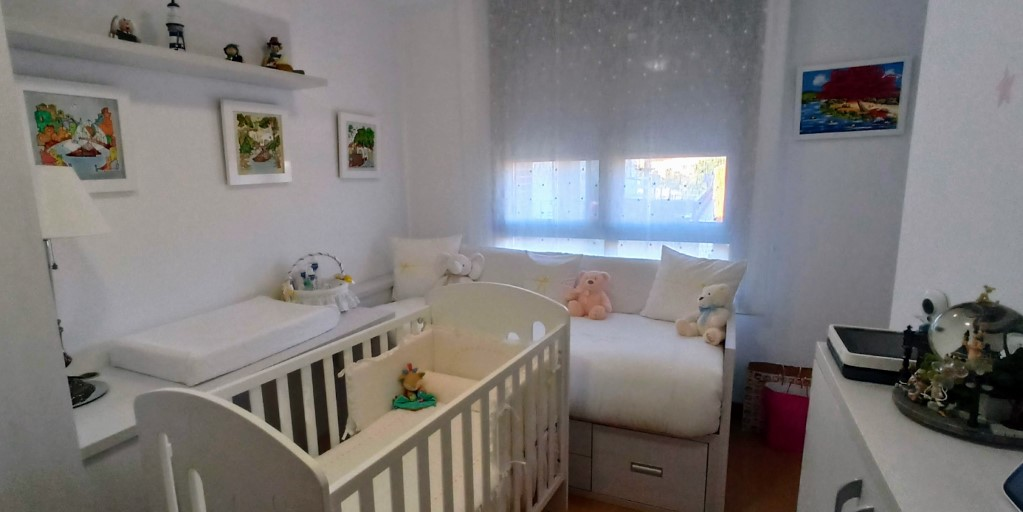
\includegraphics[width=0.85\textwidth]{./figuras/setup_bebe.jpg}
\caption{Setup 2023.}
\label{F:setup_bebe}
\end{center}
\end{figure}
El final de la pandemia reinicio los planes familiares paralizados. Como conclusión aun con la mejora sustancial del setup y sus deficiencias era necesario conseguir una alternativa real en un periodo de 12 a 18 meses incluyendo un nuevo lugar o habitáculo para el setup. Ya que a finales de 2022 el aspecto de la habitación-teletrabajo pasó a ser el siguiente:


\subsection{Nueva habitación}\label{S:nueva_room}
Vivo en un ático de 90 {\rm$m^{2}$}, desgraciadamente la disposición espacial no es eficiente ( 75 {\rm$m^{2}$} útiles) y siempre hace falta espacio de almacenamiento. La predisposición del salón o habitaciones no facilitan la instalación de una zona de trabajo, por lo que no es posible, sin dedicar una habitación en exclusiva.

En primer lugar de interés al igual que muchos amantes del bricolaje es “el trastero”, ya que unos escasos 2-6 {\rm$m^{2}$} predispuestos son más que suficientes para nuestras necesidades, sin embargo, los pisos de mi bloque no cuentan con trasteros propios, por lo que coloque una caseta de pvc en la terraza que realiza dichas funciones de almacenaje.

El segundo lugar de interés ampliamente utilizado en ciudades como Barcelona, Castelldefels o Gava, son los balcones y galerías. Espacio estrechos pero alargados fácilmente convertibles mediante cerramiento de aluminio acristalado para conseguir un espacio extra. Aunque cuento con un amplio balcón-terraza de 10 {\rm$m^{2}$}, la normativa de mi municipio no permite su cerramiento, ya que contiene una escalera de caracol que da acceso directo a la terraza superior.

Tercero, cerramiento de parking o estructura metálica sobre el parking. Dependiendo de las dimensiones acceso y altura del parking, es posible dedicar ciertos metros a una diminuta habitación mediante cerramientos simples o la instalación de estructuras metálicas con el objetivo de obtener la superficie de parking en vertical para la instalación de un trastero. La normativa comunitaria y especialmente la aseguranza de la misma no permiten la instalación de dichas estrategias ni lugares cerrados de almacenaje, por riesgo de incendio.

\begin{figure}[!htb]
\begin{center}
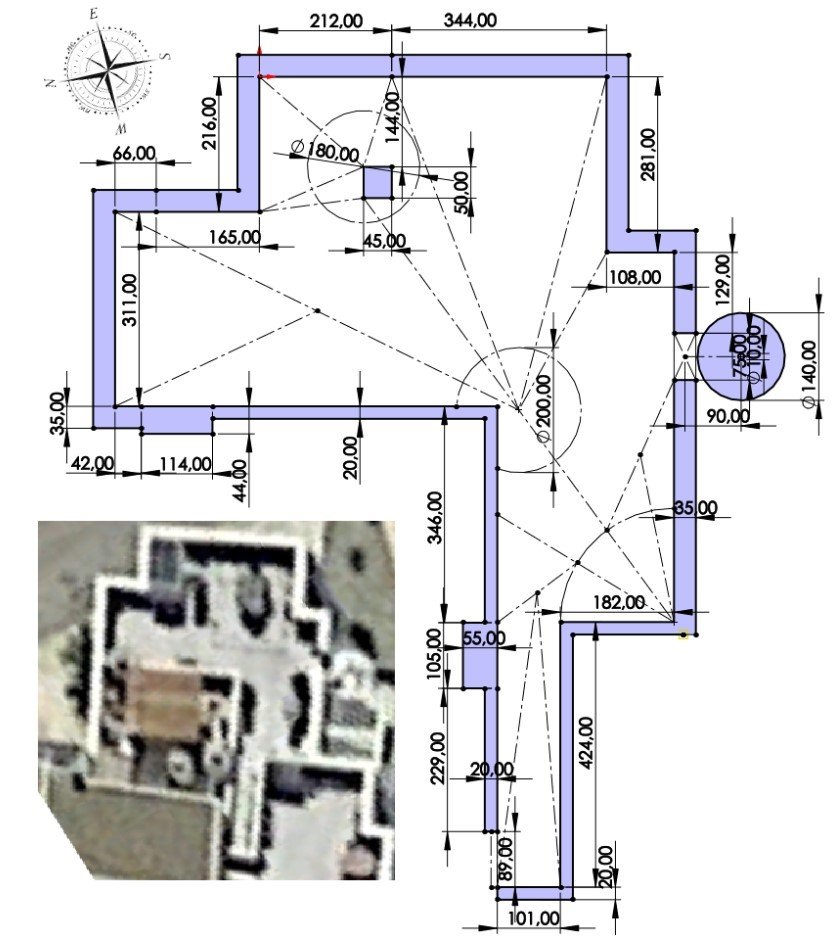
\includegraphics[width=1\textwidth]{./figuras/terraza.jpg}
\caption{Terraza planos, pendiente y zonas inúndales.}
\label{F:terraza}
\end{center}
\end{figure}

Finalmente al ser ático, dispongo de una amplia terraza, algo mayor que el 50\% de la superficie del piso (50-60 {\rm$m^{2}$}) que sin embargo, debido a su predisposición en “L”, un pasillo de acceso y una chimenea-respiradero en la parte principal más ancha, no tiene un uso práctico mayor a 35 {\rm$m^{2}$}, donde el drenaje de la misma es muy deficiente con zonas inúndales marcadas en círculos en el plano (fig.\ref{F:terraza}) que indica las pendientes de drenaje. Además es una terraza comunitaria de uso privativo, es decir, que de acuerdo a las normativa municipal y la ordenanza comunitaria, no se pueden instalar ningún tipo de elemento que:
\begin{itemize}
    \item Se fije o taladre al suelo comunitario.
    \item Rompa la estética (color) del edificio (blanco) y grises (baldosas).
    \item Medianeras, pérgolas,  mobiliario de terraza deben ser del tipo, color y dimensiones establecidas en las reglas comunitarias.
    \item Deben ser elementos de carácter no fijo (desmontables), barbacoas, barras, armarios o cerramientos únicamente anclados en paredes o alféizares.
\end{itemize}

Como especial interés, se definieron las separaciones de medianil, por paneles de aluminio lacado blanco, fuertemente anclados en los muros. Permitiendo cubrir muros vecinales o espacios entre paredes y chimeneas, siempre y cuando hubiese consentimiento mutuo entre vecinos y no se anclaje nada en fachada o paredes comunitarias.

\subsection{Caseta Oficina}
A veces las soluciones son una combinación de casuística y defectos utilizados a tu favor. Durante la pandemia intentamos solucionar los problemas de la terraza, falta de privacidad, una gran cantidad de espacio infra usado y las continuas inundaciones de la caseta-pvc usada como trastero. Así mismo la instalación del PLC y el “trabajo desde exterior” me dejó claro que con el cerramiento adecuado, era el lugar perfecto para trabajar.

\begin{figure}[!htb]
\begin{center}
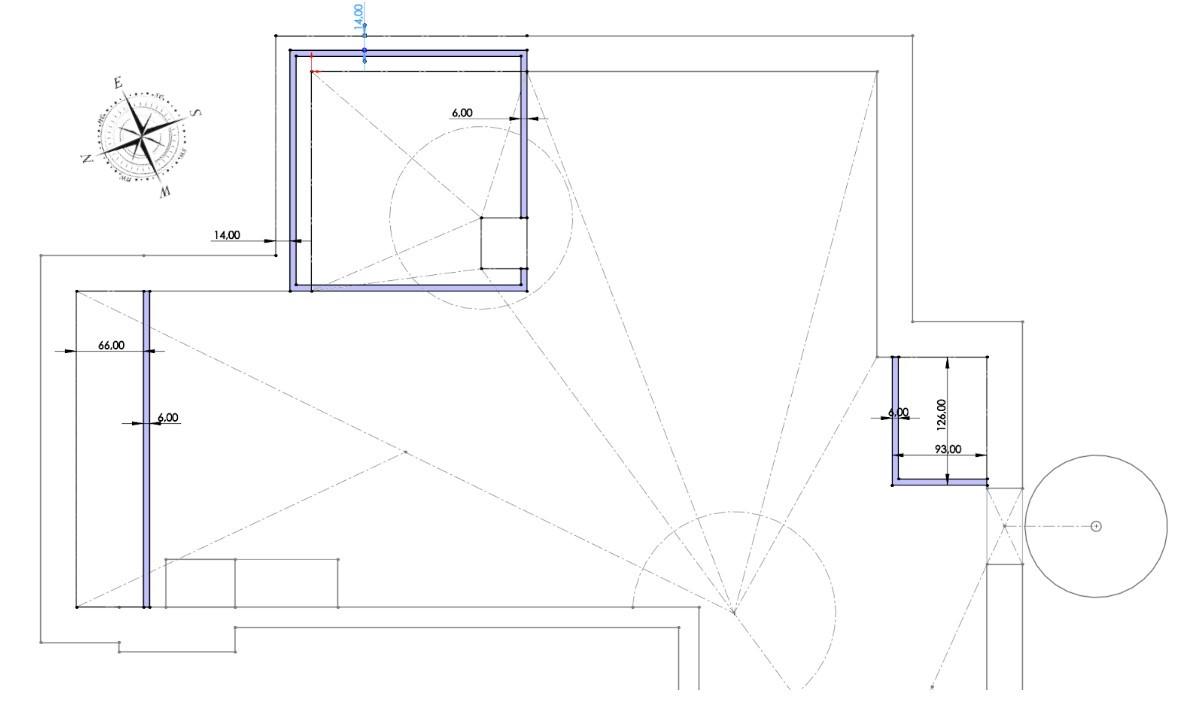
\includegraphics[width=1\textwidth]{./figuras/cerramiento.jpg}
\caption{Terraza cerramientos planificados  con pendientes zonas inúndales marcadas.}
\label{F:cerramiento}
\end{center}
\end{figure}

El plan se basaba en cerrar el medianil con el separador de aluminio para ganar privacidad y que el mismo proveedor de aluminio nos hiciera un armario-almacenaje en torno a la zona no inúndable de espacio muerto entre barbacoa y pared norte. Sin embargo no se llegó a entendimiento con el vecino. 

\begin{figure}[!htb]
\begin{center}
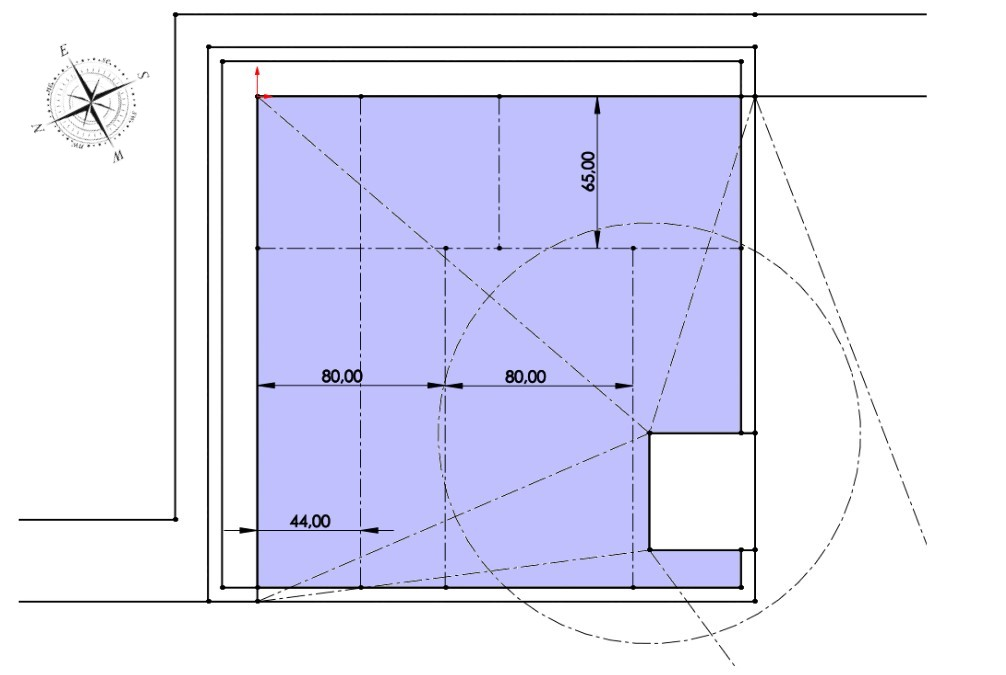
\includegraphics[width=0.85\textwidth]{./figuras/caseta_division_spacio.jpg}
\caption{Caseta división espacial.}
\label{F:caseta_division_spacio}
\end{center}
\end{figure}
Entonces comente la idea de similar al armario, rehacer la caseta-trastero de PVC, pero utilizando el material de separación entre vecinos. El objetivo inicial era conseguir una caseta hermética, evitando “el charco” y el moho, pero sobre todo ganando el alféizar como espacio útil y permitiendo colocar estantes en él, con el fin de obtener un pseudo trastero.

Al detallar, descubrimos que lo que normalmente es 1.80 m de altura, debido a la mala colocación de terraza y a un alféizar algo elevado, los puntos de anclaje de la futura caseta permitían unos valores de 1.86-1.89 m respecto al suelo real de la terraza, es decir, un lugar donde a mi altura 1.79, permite moverse como en una habitación de techos bajos. 

Por otra parte la chimenea-respiradero, pasa de ser un elemento problemático, a un elemento estructural, que permite anclar y dar robustez al formar un cuadrado entre muro-alféizar y chimenea, permitiendo el anclaje lateral y en conclusión resistir cualquier tipo de vientos al cerramiento de aluminio. Por otra parte interiormente habilita un pared robusta sobre la  que anclar elementos como pizarra o mini estanterías.

\subsubsection{Trabajos previos}\label{S:trabajos_previos}
Durante los meses previos a la instalación de la caseta se realizó una limpieza completa de las zonas afectadas. La limpieza de alféizar, pared y suelo con agua a presión, posteriormente con bases ácidas vinagre blanco (alféizar) y salfuman (baldosas) para la eliminación y apertura de poros.

\begin{figure}[!htb]
\begin{center}
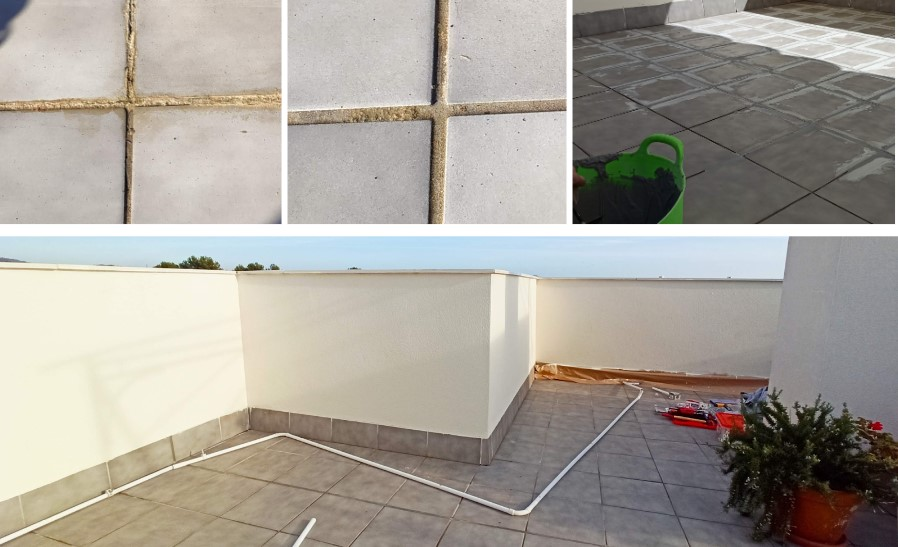
\includegraphics[width=1\textwidth]{./figuras/trabajos_previos.jpg}
\caption{Limpieza, pintura y trabajos previos.}
\label{F:trabajos_previos}
\end{center}
\end{figure}

Así como una adecuación de la instalación eléctrica con la instalación de canalizaciones, cableado y respectivas cajas con el fin de mejorar y separar completamente iluminación de terraza, enchufes húmedos, electricidad de la oficina y cable ethernet.

\begin{figure}[!htb]
\begin{center}
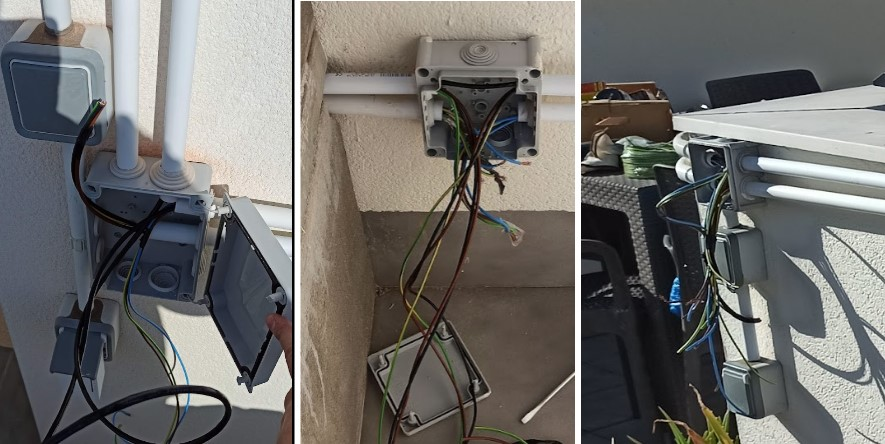
\includegraphics[width=1\textwidth]{./figuras/trabajo_electrico.jpg}
\caption{Montaje de sistema eléctrico y cableado Ethernet.}
\label{F:trabajo_electrico}
\end{center}
\end{figure}

\subsubsection{Estructura, aislamiento y estanqueidad} \label{S:estructura_aislamiento}
La estructura y el aislamiento viene de la mano de paneles sándwich de aluminio, al igual que la separación entre vecinos se basan en anclajes verticales, que unen los paneles de aluminio cada 1.5-2 metros. 
\begin{figure}[!h]
\begin{center}
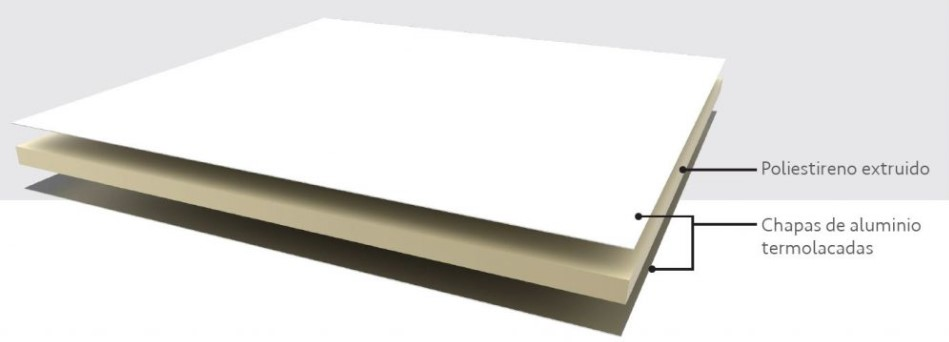
\includegraphics[width=1\textwidth]{./figuras/panel_aluminio.jpg}
\caption{Panel de aluminio lacado con aislante térmico.}
\label{F:panel_aluminio}
\end{center}
\end{figure}
\begin{figure}[!h]
\centering
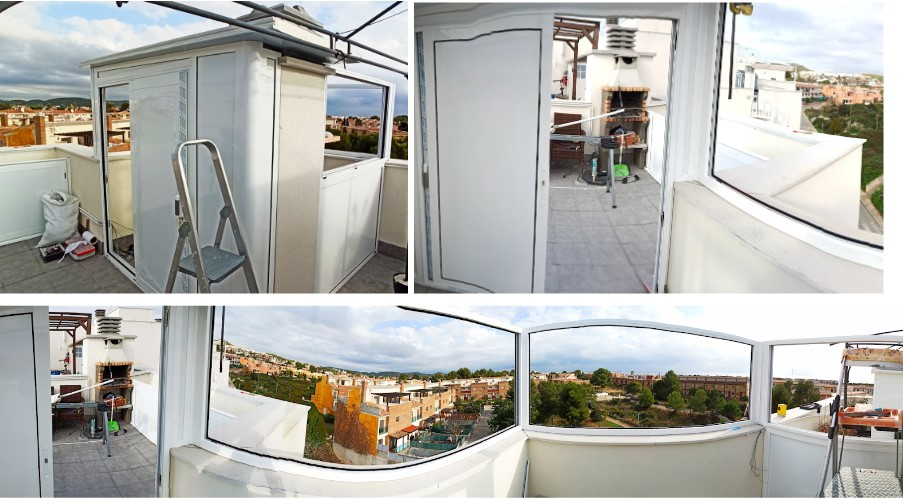
\includegraphics[width=1\textwidth]{./figuras/montaje_aluminio.jpg}
\caption{Montaje paneles aluminio y soportes.}
\label{F:montaje_aluminio}
\end{figure}
\begin{figure}[!h]
\centering
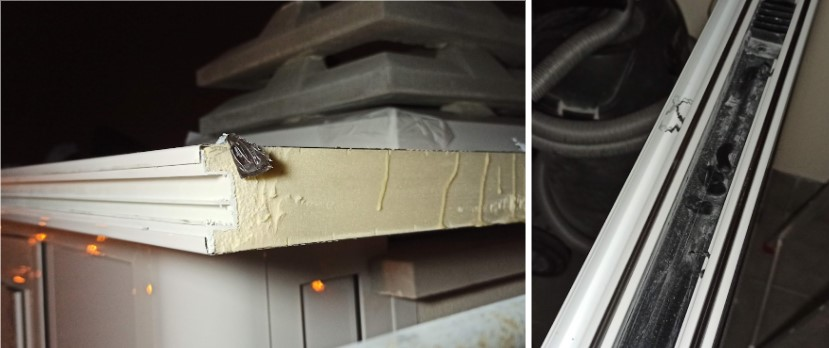
\includegraphics[width=1\textwidth]{./figuras/perfil_aislamiento.jpg}
\caption{Vista de perfiles y techo con aislamiento.}
\label{F:perfil_aislamiento}

\end{figure}
La estrategia se basa en utilizar paneles más grueso de 4 cm para un mayor aislamiento, especialmente en tejado 7 cm, ya que la incidencia solar es directa y prolongada durante los meses de verano. Estos paneles, son sujetados por premarcos de aluminio (similares a ventanas) que a su vez se fijan directamente sobre alféizar, paredes o perfiles estructurales en las esquinas. 
Todos ellos entre sí, así como los elementos que se fijan quedan perfectamente sellados por siliconas especializadas, incluido la base del perfil en contacto con el suelo de la terraza.

\subsubsection{Instalación interna y montaje mobiliario}
Una vez terminados los trabajos de instalación de los cerramientos y el apropiado secado de los mismo, se inició un montaje tanto de cajas, enchufes e interruptores eléctricos de ambos cerramientos
\begin{figure}[!htb]
\begin{center}
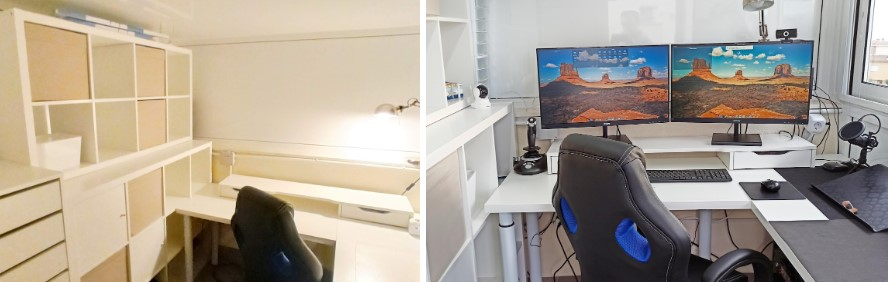
\includegraphics[width=1\textwidth]{./figuras/caseta_mobiliarioysetup.jpg}
\caption{Mobiliario y setup en caseta.}
\label{F:caseta_mobiliarioysetup}
\end{center}
\end{figure}
Junto con una migración del setup validando tanto conectividad, enchufes e iluminación, permitiendo comenzar el teletrabajo desde la oficina conforme se van añadiendo más elementos complementarios necesarios especialmente relacionados con temperatura e iluminación.
\begin{figure}[!htb]
\begin{center}
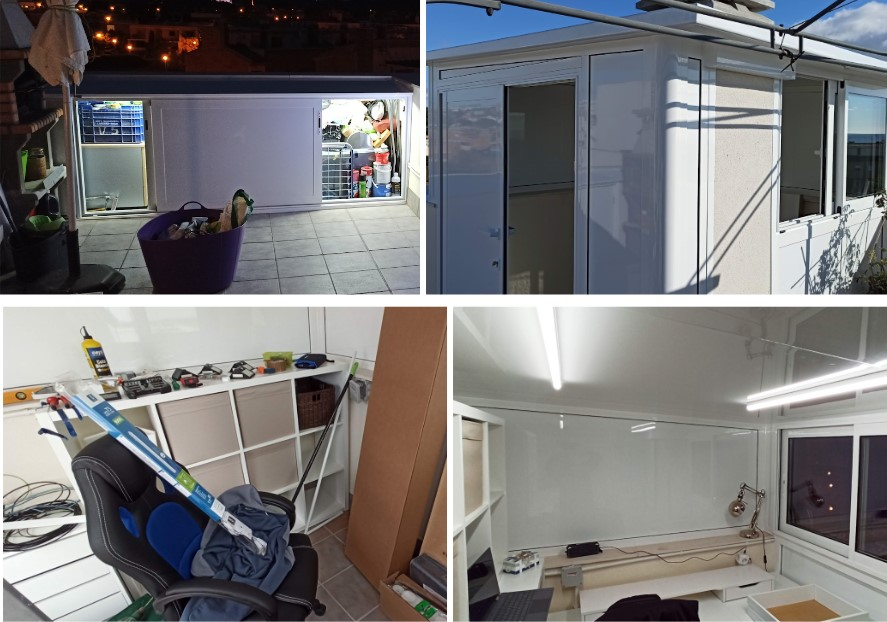
\includegraphics[width=1\textwidth]{./figuras/caseta_electricidad.jpg}
\caption{Instalación eléctrica en caseta y cerramientos.}
\label{F:caseta_electricidad}
\end{center}
\end{figure}

\newpage
\subsubsection{Aclimatación e iluminación}\label{S:iluminacion_caseta}
El primer elemento necesario de la “hermética caseta” es la instalación de varios respiraderos naturales para la circulación de aire, siendo estos fácilmente operados manualmente para evitar la entrada de frío/calor en circunstancias adversas.

 Aunque el aislamiento bastante sobredimensionado para un cerramiento usual, no deja de ser 4-7 cm similar a una puerta de parking, es decir, bastante útil para evitar el calor directo pero insuficiente en invierno para evitar la bajada de temperaturas. Por otra parte tanto el muro como el suelo original son elementos fríos, que permanecen a la temperatura de la estructura del edificio, algo fresca en verano pero fría en invierno.

 Por lo tanto se han instalado alfombras (duras y gruesas) junto a un calefactor eléctrico, así como ventiladores pingüino de bomba de calor aire frío/calor.

 \begin{figure}[!htb]
\begin{center}
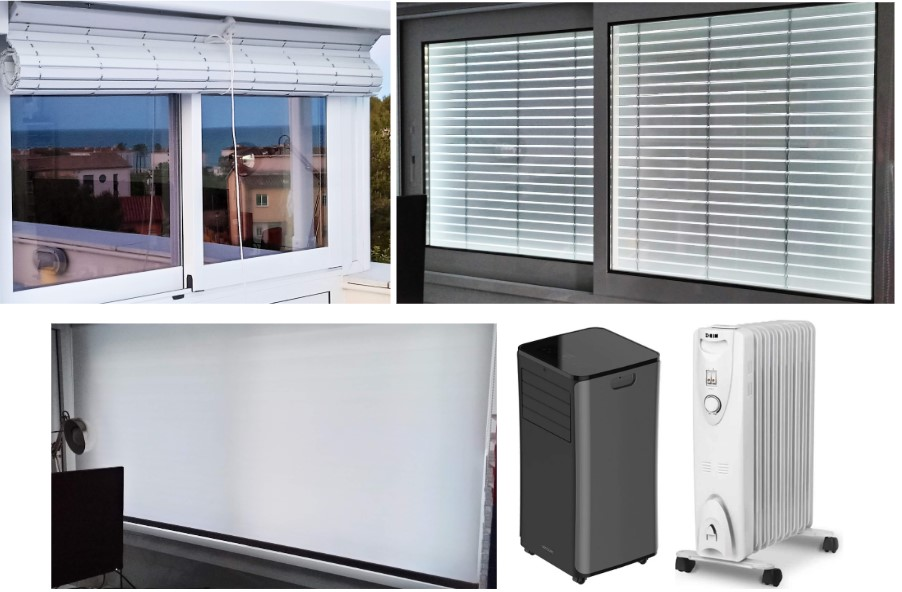
\includegraphics[width=1\textwidth]{./figuras/luz_regulacion_termica.jpg}
\caption{Regulación térmica y lumínica.}
\label{F:luz_regulacion_termica}
\end{center}
\end{figure}

Finalmente la ventana se ha utilizado un cristal especial, que minimiza la entrada de calor por vía solar, especialmente intensa en verano, que a su vez debido también al fuerte reflejo directo continuado por la vista directa al mar, ha obligados a la colocación tanto de un estor difusor de luz, así como una alicantina externa con el objetivo de reducir sustancialmente la intensidad y la dirección lumínica de la luz natural.

\subsection{Mejoras de Terraza}
A continuación se han realizado varias mejoras a la terraza que aunque no tiene conexión directa con la “oficina-caseta” influyen positivamente en la misma.

\begin{figure}[!htb]
\begin{center}
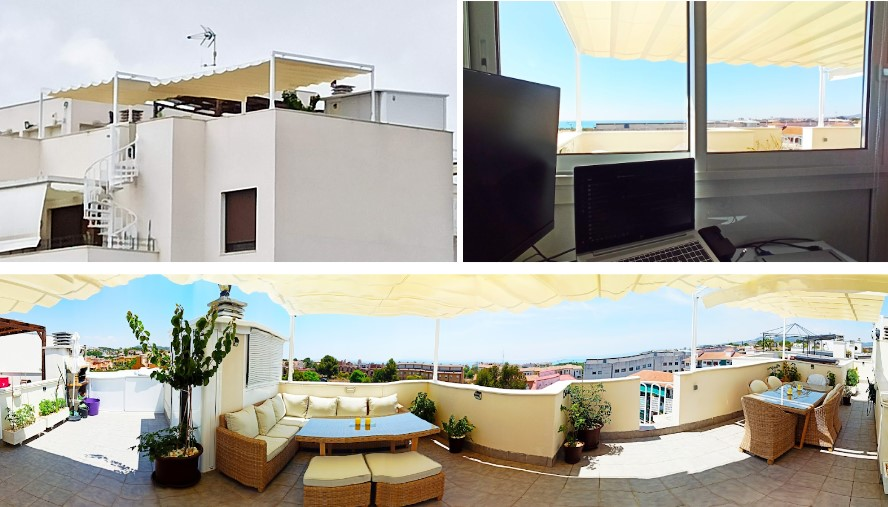
\includegraphics[width=1\textwidth]{./figuras/mejoras_terraza.jpg}
\caption{Mejoras externas de terraza que afectan a la caseta.}
\label{F:mejoras_terraza}
\end{center}
\end{figure}
Una de las grandes desventajas de la terraza es su nulo uso entre junio-septiembre debido a la alta intensidad lumínica y de calor, debido al número de horas de luz directa más el reflejo del mar. Con el objetivo de mejorar su uso, así como reducir la temperatura del suelo y reducir el calor que transmite al ático, se implementado dos toldos corredero de grandes dimensiones, que junto a una vela triangular y una sombrilla, permiten cubrir el 80\% de la terraza en sombra las principales horas del dia 11-17, así como provocan una zona en sombra tanto a la paredes de la caseta como parcialmente en el tejado de la misma.

\begin{figure}[!htb]
\begin{center}
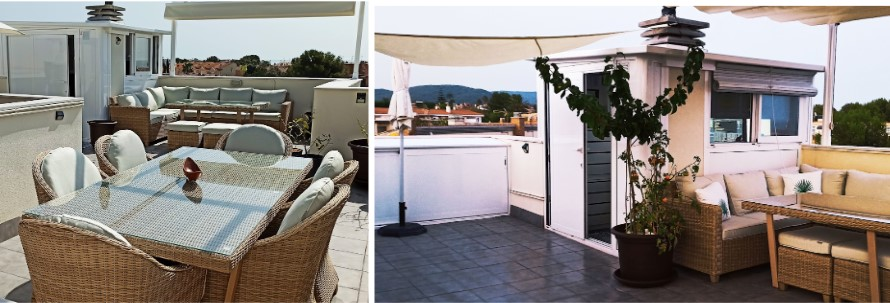
\includegraphics[width=1\textwidth]{./figuras/mejoras_terraza_2.jpg}
\caption{Mejoras externas de terraza II que afectan a la caseta.}
\label{F:mejoras_terraza_2}
\end{center}
\end{figure}

Por otra parte se ha renovado el mobiliario exterior, la distribución del mismo, permitiendo salir al exterior de manera cómoda cuando las condiciones climáticas y lumínicas lo permiten.

\section{Evaluaciones, mejoras y correcciones}\label{S:cambios_2023}
Por otra parte se han detectado mejoras realizadas sobre el diseño original así como estrategias fallidas durante 2022-23 que han requerido de arreglos o un cambio radical en la solución final.

\subsection{Humedades y condensación}
Aunque el hermetismo del cerramiento es perfecto existen dos fuentes de humedades resueltas parcialmente. 

La principal son el alféizar y muros originales del propia cerramiento, aunque están debidamente pintados con pintura transparente anti-humedad, esta capa únicamente limita la salida o la evaporación de la humedad, permitiendo que aquellas semanas con 3-6 días de lluvias continuadas la humedad progrese por la pared hasta llegar al zócalo por donde aparece en forma de superficie húmeda.

Las juntas entre las baldosas, como se ha explicado el cerramiento se sitúa sobre un punto más bajo que el resto de la terraza, esto junto a la porosidad tanto de baldosas como de juntas, promueve un lento avance de humedades los días de lluvia,y de igual manera cuando supera los 2-3 días comienza no solo a “humedecer” sino a acumular 1-3 mm de agua.

\begin{figure}[!htb]
\begin{center}
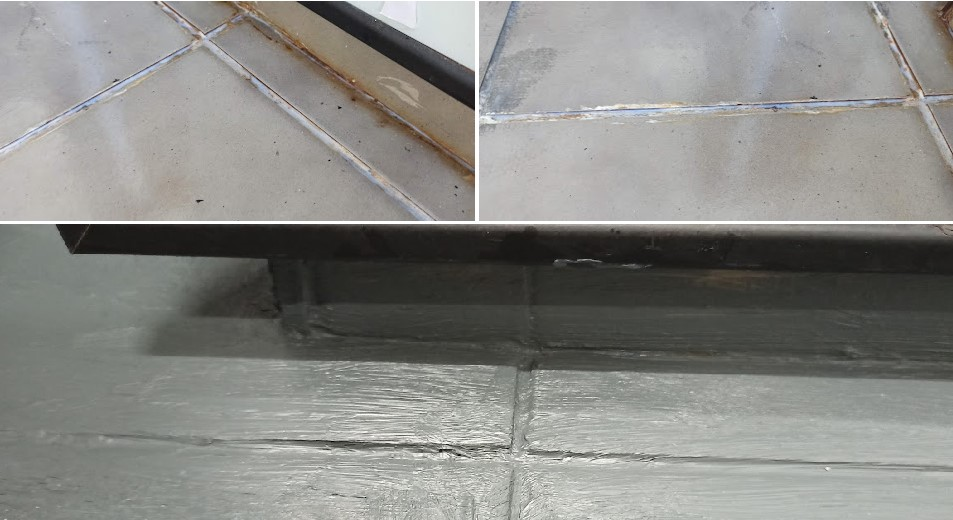
\includegraphics[width=1\textwidth]{./figuras/humedades.jpg}
\caption{Impermeabilización con pintura y silicona.}
\label{F:humedades}
\end{center}
\end{figure}

La solución de ambos problemas ha sido múltiples capas de pintura anti-humedad junto a el uso de silicona líquida para sellar completamente tanto suelos como zócalos o posibles entradas de agua por porosidad o capilaridad.

Otro problema recurrente es el propio hermetismo de la sala, si se cierran los orificios de ventilación en invierno con la finalidad de mantener la temperatura. Cualquier humedad interna, especialmente el propio vapor humano, termina condensando en los paneles de aluminio o ventanas, cuya única solución es ventilar intervalos de 3-5 horas, con especial interés previos a la noche.

\subsection{Bomba de calor/frío}\label{S:cambios_bombacalor}
El uso del “pingüino” para calentar, enfriar o des humidificar ha sido un completo fracaso. Aunque la potencia del mismo es para habitaciones de 15 {\rm$m^{2}$} (ampliamente sobredimensionado), el caudal de aire entrante-saliente necesario para su funcionamiento hace ineficaz su uso debido a las pequeñas dimensiones de la habitación.

Enfría / calienta un aire que se renueva rápidamente 10-20\%, es decir, que gran parte del movimiento térmico realizado, se utiliza para re-aclimatar el aire nuevo, no permitiendo subir de los 21º en invierno (12-17º exterior), o bajar de 24º en verano (28-33º exterior), a su vez esta renovación de aire trae consigo humedad que el sistema debe retirar, es decir está continuamente eliminando humedad, que debido a al mal drenaje de la terraza se convierte en un charco o un recipiente a vaciar manualmente.

La reducción u obstrucción de la ventilación para reducir el caudal de aire exterior soluciona parcialmente el problema pero convierte la pequeña y hermética caseta, en una sala de presión negativa, sobre esfuerza el motor que expulsa el aire, estresa la estructura de aluminio y genera “silbidos”  por la presión negativa en la puerta corredera. 

Por último su mayor problema es que su uso continuado genera excesivo ruido tanto para vídeo conferencias, dificultando la concentración e incluso generando dolor de cabeza. La humedad es un problema especialmente dañino en verano puesto que aunque la temperatura generada dura 90-120 minutos debido al aislamiento, la humedad se re-equilibra con el exterior rápidamente en cuestión de 15 minutos.

Finalmente la realidad ha sido que la desmantelación total de la bomba de calor y el uso de elementos más rudimentarios tales como un calefactor eléctrico tradicional o el uso de la brisa veraniega combinada con ventiladores, satisfacen de una manera más adecuada y sin problemas (ni el gasto eléctrico sobredimensionado).

\subsection{Paneles solares y SAI}
La desaparición de la bomba de calor portátil ha proporcionado un espacio debajo de la mesa útil para la generación de un SAI casero, véase figura \ref{F:instalacion_electrica} donde se predispone la batería y generador de alterna contiguo a un conjunto de enchufes. 

Con el objetivo de disponer de una fuente de energía alternativo para el setup, así como permitir la alimentación tanto de ventiladores, calefactores eléctricos o servidores autocráticos se ha instalado una batería solar de 128 AH a 12 V de ciclos profundo junto con la instalación de paneles solares que alimentan el sistema.

\begin{figure}[!htb]
\begin{center}
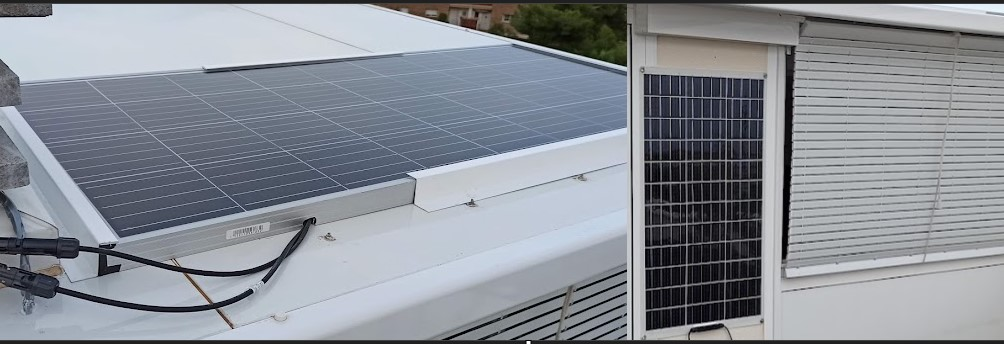
\includegraphics[width=1\textwidth]{./figuras/panel_solar.jpg}
\caption{Paneles solares, tejado y frontal chimenea.}
\label{F:panel_solar}
\end{center}
\end{figure}

Se ha predispuesto de un panel solar de 160 W orientado a  sur en el tejado, cuya eficiencia se ve lastrada por la inclinación del mismo (5º), pero permite una captación de luz permanente durante el 80\% de las horas diurnas, así como el reflejo y dispersión atmosférico. Permite captar 0.5-2 A durante las horas mínimas(6-24w), 6-7A al medio día en invierno y 10-11 A en verano, es decir, entorno 80-130W. Así mismo con el objetivo de compensar la  horizontal y el cambio de posición solar invierno/verano se ha instalado un panel de 100W de alta eficiencia en paralelo en orientación sur vertical, que aparte de la luz directa, recibe de manera constante y directa el reflejo marino durante todo el día.

La conjunción de ambos paneles generan un flujo constante y complementario de corriente, compensando tanto la inclinación solar durante las estaciones, como su transito durante el día. Buscando un suministro constante de 30-50W en las peores condiciones y picos de productividad 150-170W durante el medio día soleado.

La principal función de este sistema es un uso constante de los sistemas ambientales, ventiladores en verano (5w, 5w, 25-50w), el uso de calefactores en invierno 150 w, así como el almacenaje de la energía no utilizada para la funcionalidad de SAI, proporcionada por un generador continua-alterna de 1000W, fácilmente conmutable para alimentar pantallas y laptop en periodo de 4-6 horas.

\subsection{Domótica y alarma}
Durante 2023 he implementado diversos mecanismo de domótica y seguridad en mi vivienda. Entre ellos la instalación de:
\begin{itemize}
    \item Sensores de presencia, sensores magnéticos (puertas, ventanas), sensor de humo/gas, sensor temperatura / humedad, detectores de presencia  y termostato inteligente.
    \item Alarma con batería y conexión 3G / wifi, usando aplicación genérica de domótica y API de eventos.
    \item Actuadores tales como bombillas inteligentes, enchufes inteligentes, regletas y conmutadores inteligentes, PIA inteligente, diferencia rearmable.
    \item Interfaces humanas, smart tv, amazon alexa, google eco.
    \item Gateways de zigbee, z-wave, wifi, bluetooth y 144 Mhz.
    \item Cámaras Ip fijas, o con actuadores.
    \item Rasberry pi con home assitand y API configuradas (google, alexa y gautone).
\end{itemize}

Aunque son elementos asociados a la vivienda y automatizados en mis cuentas personales, afectan a la oficina automatizado el encendido y apagado de elementos tales como climatización, monitorizando terraza o interior de caseta (cámaras y sensores de temperatura y humedad) así como proveen una seguridad y notificación efectiva del área de trabajo.
